\documentclass[12pt]{article}
\usepackage{amsmath}
\usepackage{hyperref}
\usepackage{url}
\usepackage[onehalfspacing]{setspace}
\usepackage[top=2.5cm, bottom=2.5cm, left=2.5cm, right=2.5cm]{geometry}
\usepackage{mathptmx}
\usepackage{enumitem}
\usepackage[style=ieee]{biblatex}
\usepackage{xcolor}
\usepackage{listings}
\usepackage{dirtree}
\usepackage{tabularx}
\usepackage[automake]{glossaries-extra}
\usepackage{graphicx}
\usepackage{float}


\hypersetup{
      colorlinks=true,
}
\setlist{nosep}

\makeglossaries


\newglossaryentry{llvm}
{
    name=LLVM,
    description={LLVM (originally standing for Low Level Virtual Machine) is a system
    of compilers and toolchains and software to create them.}
}

\newglossaryentry{taggedUnion}
{
    name={tagged unions},
    description={Tagged Unions are types whose values can contain several different
    types of which the current type is signified by a value (the tag).}
}

\newglossaryentry{sugar}
{
    name={syntax sugar},
    description={Syntax sugar is a convenient way to write something, but is technically redundant.}
}

\newabbreviation{ir}{IR}{Intermediate Representation}
\newabbreviation{wasm}{WASM}{Web Assembly}
\newabbreviation{vscode}{VSCode}{Visual Studio Code}
\newabbreviation{gc}{GC}{Garbage Collector}
\newabbreviation{api}{API}{Application Programming Interface}
\newabbreviation{ffi}{FFI}{Foreign Function Interface}
\newabbreviation{adt}{ADT}{Algebraic Data Type}

\addbibresource{bibliography.bib}


\title{Creation of a functional programming language\\matura project}
\author{Enea Giger\\Supervisor: Adrian Lüthi}
\date{Gymnasium Burgdorf\\\today}


\newcommand{\importListing}[1]{
    \begin{minipage}{\textwidth}
    \input{#1}
    \end{minipage}
}

\begin{document}
\maketitle
\begin{figure}[h]
	\centering
	\begin{tabular}{c}
		\begin{lstlisting}[basicstyle=\tiny]
             ##
             ##
          # #####
          #########
         ##########
         ##########
    ### ###########
   ################
##################
   ################
    ### ###########
         ##########
         ##########
          #########
          # #####
             ##
             ##
\end{lstlisting}\end{tabular}
	\caption{The Mandelbrot Set computed by the program at \file{examples/mandelbrot.imp}}
\end{figure}


\begin{abstract}
	This paper describes a new functional programming language called Imp
	which is strictly typed, but does not need explicit type annotations by the
	developer. The language is kept simple, deliberately having a small set of expressions and statements.
	It describes its implementation by creating an interpreter and a compiler from scratch,
	two entirely seperate methods for executing the code.
	These implementations are written almost exclusively in the systems language
	Zig.
	The paper describes in detail the architecture and algorithms used by the
	implementations. Notably, a method for tail call optimization was used
	to enhance the performance of the interpreter. The compiler includes
	a transformation from Imp to \Gls{llvm} \gls{ir},
	which in turn is used for compiling to executable machine code.
\end{abstract}
\newpage

\tableofcontents
\newpage

\section{Introduction}
In todays world, computers are omnipresent. In our service-oriented society,
almost everything depends on applications we run on them.
And all these applications have to be written in some programming language,
nowadays in most cases imperative or general-purpose ones like C++, JavaScript or Python.

Functional programming is another paradigm used by languages like Haskell, Standard ML and Erlang
which are often used in programming language or mathematical research,
but are much less popular outside of academia.
The functional approach proves to be well suited for problems which involve parallelism,
meaning several processes that must run at the same time,
shown in practice by Erlangs usage in WhatsApp and Discord.
They are called functional because they are based on mathematical functions,
which given the same input, result in the same value each time.
This is in contrast to imperative programming languages whose functions are
actually procedures, meaning step by step instructions of what to do
and whose results depend not only on the input, but on the current state, which they
might change. These changes are called side effects, which are not allowed in purely
functional languages.
Instead of constructs like loops, recursion is used in functional languages similar to mathematics.
Functional programming languages also have first-class functions, meaning
all functions are values and can therefore be passed around to other functions
or stored in variables.
The functions in functional programming are also closures, which means they
can enclose values present at the time of their creation.
This means that if functions are created inside another scope
they still work outside of that scope even if they access local variables.
Scopes are parts of a program in which variables can be defined until
the scope ends, after which the access to these variables is no longer possible;
scopes define the lifetime of variables.



The main goal of this project was to devise a functional language
and create an implementation, starting with a simple interpreter.
The principal aim for the syntax of the language was also to keep it small,
so the focus could lie more on the implementation instead of language design.
To that end it had to have strictly immutable variables and have no looping constructs.

The language was later decided to be called Imp as in impure, imperfect, and implementation.

\newpage
\section{Fundamentals}
Though programming languages can be very different in appearance and paradigms,
the elementary steps taken in each implementation are
still mostly the same for all languages, whose functions need to be understood
and which are introduced below.

\subsection{The Lexer}
The first step of a programming language implementation is almost always the lexer.
It is responsible for splitting up the source code into tokens,
which are little chunks such as the name of a variable or the name of a statement,
but also grouping elements like brackets.
Essentially, for natural languages, the tokens would be the words and punctuation.
These tokens can then be used as input for the parser.

\subsection{The Parser}
After the lexer, the parser of a programming language is responsible
for ensuring correct syntax and, in most cases,
building a tree out of the tokens, called the syntax tree which is a representation
of the code in memory more suitable for further transformation or execution.
This can be done in many ways, though what methods are applicable
depend on the syntax of the language.

\subsection{Type Checking/Inference}
After the program has been parsed,
a semantic analysis step follows if needed.
This step often consists of a type checker.
The type checking step ensures that programs are correct
regarding the type system of the language.

Type systems can be type-safe or not.
If a language has a type-safe type system, programs in that language
must be well-typed, meaning only operations that can be done safely are applied
so no runtime type error can occur as they can in dynamically typed
languages like Python or in languages that allow unsafe type conversions like C.
Languages with type safe type systems are often called
strongly typed, while non-type-safe languages are called weakly typed.

A type system known to be type-safe is the Hindley-Milner type system,
originally developed for the functional programming language ML.

\subsubsection{Hindley-Milner type inference}
The Hindley-Milner type inference algorithm, as described by Damas and Milner
\autocite{damasPrincipalTypeschemesFunctional1982}
is originally a way to determine types for functions in a
polymorphic lambda calculus with an addition of let expressions.

Polymorphism is the ability of values to have different types. This
is useful as it enables having one function doing a simple task that does not
really depend on the actual type, like functions that work on lists, but do not
care what type the elements of the list have.

\paragraph{Lambda Calculus}
The Lambda Calculus is a simple model for computation introduced by Alonzo Church in 1932
\autocite{churchSetPostulatesFoundation1932}.
It is known to be
able to simulate the well-known turing machine \autocite{turingComputabilityLdefinability1937} and as such,
all implementations of the lambda calculus are turing complete.
The only expressions that are possible are:
\begin{itemize}
	\item $\lambda x.\:e$,
	      which results in an unnamed function where $x$ is the name of the argument
	      and $e$ is an expression whose value is returned if the function is called
	\item $x$, where $x$ is the name of a variable
	      and the result is the value of that variable
	\item $e_1\:e_2$, where both $e_1$ and $e_2$ are expressions and the result
	      is the result of the call of function $e_1$ with argument $e_2$\item $c$, where $c$ is a constant
\end{itemize}

For the Hindley-Milner type inference algorithm to work,
$let\:x = e_1\:in\:e_2$ is introduced, where x is the name of the variable
which is defined to be the result of expression $e_1$
and the whole expression results in expression $e_2$,
when $x$ is substituted by $e_1$.
As such the let expression is almost equivalent to $(\lambda x. e_2)\:e_1$.
The reason the let expression is needed is because polymorphism is constrained
to such variables, enabling the algorithm to always infer the types
in a well-typed program.

\subsubsection{The Inference Algorithm}
The Hindley-Milner type inference algorithm determines the most general types of expressions possible
in this variation of lambda calculus by first assuming a maximally generic type and refining it step by step
using information including the operations used (e.g. function calls).

The types it assigns are:
\begin{itemize}
	\item $a$, where $a$ represents any type and is called a type variable
	\item $P$, where $P$ is any primitive type like Int or Float, and
	\item $\tau \rightarrow \tau$, where $\tau$ is any type, representing
	      a function with the type of its argument and result
\end{itemize}

Finally the type assigned to a let can also be
$\forall \vec{a}.\:\tau$. The $\vec{a}$ is a vector consisting of
several type variables. This type means that the value assigned
can have the type $\tau$, no matter what the value of the variables contained in $\vec{a}$ are.

Refining the type is done through a procedure called unification,
which tries to find possible substitutions for type variables that would make two
types equal. This is done for instance when inferring the type of a call,
as the type of the function being called must match
the type of its argument.
If there is no way to substitute type variables
to unify the two types, the program is not well-typed.

\subsection{The Optimizer}
The next step for most language implementations is an optimizing step based on
either the syntax tree or an intermediate representation generated before.
This is done in a succession of (possibly many) optimizing passes over the representation
in most languages. The type of optimizations
possible depend on how the program is executed, whether the language is typed,
sometimes also depending on the target machine and many other aspects.

\subsection{The Interpreter}
The interpreter is the next step in many programming languages.
It is a program intended to run the user-written program.
There are many types of interpreters:
\begin{itemize}
	\item \textbf{Byte-Code Interpreters}, which run a
	      a custom-defined intermediate representation that is similar to how
	      machine code works, but more specific to the language. Most interpreted languages
	      use one, because it is most often the fastest possibility especially
	      because big continous blocks of memory can be stored efficiently in the cache.
	\item \textbf{Threaded Interpreters}, where there is no byte sequence, but pointers
	      to functions to be called or the next instruction. This has the problem that there
	      are many calls depending on pointers calculated at run-time, also known as pointer indirections
	      being done, reducing the speed, because the memory is no longer sequential.
	\item \textbf{Tree-Walking Interpreters}, which directly evaluate the tree,
	      that has potentially more information available, but might not be optimal because of syntax
	      nodes which need to be skipped and there are more pointer indirections than
	      \textbf{Byte-Code Interpreters}
\end{itemize}
Both the byte-code and threaded interpreters also require a compiler.

\subsection{The Compiler}
The Compiler uses the representation of the program and converts it into another language or representation.
Often this representation is machine code or another intermediate representation used by an interpreter.
Programs using the machine representation are usually
faster than ones run by interpreters, as they are able to use more specific
optimizations in the CPU.

Many compilers nowadays do not directly convert the code to machine code,
but depend on a backend. One of the most popular backends is \Gls{llvm}.

\subsubsection{LLVM}
The \Gls{llvm} Project contains a backend capable of converting a language called
\Gls{llvm} \Gls{ir} into code for several targets,
like x86-based CPUs (most Intel and AMD chips), ARM-based CPUs, but also
\Gls{wasm}, which is understood by browsers.
This means that many optimizations can be reused without the need to
write them once more for each new language.

It is coded in C++, though bindings exist for several languages, most notably
for C, which many languages can interact with.

\section{Implementation}
Now that the basics have been covered, the specifics
of the implementations can be explained in depth.

\subsection{Used Software}
The Programming Language was implemented in Zig, a new low-level programming
language that aims to improve on C. Zig was used in this project since it has built-in
support for \gls{taggedUnion} and a build system. \Gls{taggedUnion} were deemed important because they
enhance type safety which helps implementing especially the syntax tree because it is ensured
that the different node types have all been covered.
However, for the compiler, C was still used for a few built-in functions.

\Gls{llvm} was used as a tool to compile Imp to machine code while the
Boehm-Demers-Weiser \Gls{gc} C library \autocite{GarbageCollector} was
used to manage memory in the compiled program.
To develop and test the conversion to \Gls{llvm} \Gls{ir}, the web page
compiler explorer \cite{godboltCompilerExplorer} was used.

The Software was developed using the Editors \Gls{vscode} and Zed.
Zed was used primarily, with \Gls{vscode} used for features like Debugging
that initially did not yet exist in Zed.

For the ability to highlight the syntax of code written in Imp, an additional parser was made using tree-sitter \autocite{brunsfeldTreesitterTreesitterV025102025}.
This parser is written in JavaScript. Since the grammar of the language is tedious to describe using
the parser functions given by tree-sitter, a custom lexer was also implemented, which itself was written in C.
To state what parts of the code should be colored how, queries had to be written as well,
which are written in an unnamed language unique to tree-sitter.
Highlighting with tree-sitter was chosen specifically since it is used
in the editor Zed, enabling a custom extension to be written for Imp.

This article itself was written in LaTeX, while the listings were generated
by chromacode \autocite{lebedaTomLebedaChroma_code2025}, reusing the tree-sitter parser.

The flow diagram included in this paper was generated using draw.io \autocite{drawioltdDrawio}.

\subsection{The Language}
\importListing{code/either.tex}
The Syntax of the language consists of statements and expressions.
\\
There are only two types of statements.
\begin{itemize}
	\item Type statements, which define an \Gls{adt},
	      meaning a type whose values can be constructed by various
	      constructors when given specific arguments.
	      These types can be generic.
	      An example can be seen in Listing \ref{listing:either}, where the type $Either$ is defined,
	      which can be constructed by either a value of type a or of type b.
	\item Let statements, which define an (immutable) variable
	      in the rest of the file. If the variable is assigned a
	      lambda expression, it can be recursive
\end{itemize}
All statements must not be indented,
whereas all expressions have to be indented.
This is the only case of significant whitespace in the language.
\\
The types of expressions (\texttt{e}) that exist are:
\begin{itemize}
	\item Lambda expressions (\texttt{lambda x.e}), which work exactly
	      the same as in lambda calculus
	\item Let expressions (\texttt{let x = e\textsubscript{1} in e\textsubscript{2}}),
	      which work the same as in the variation of lambda calculus
	      described earlier used in the Hindley-Milner type system,
	      except, as with the statement,
	      it can be recursive if assigned a lambda
	\item Variables (\texttt{x}),
	\item Function Calls (\texttt{e\textsubscript{1} e\textsubscript{2}}),
	\item Constants, meaning Integers (eg. \texttt{42}), Floats (eg. \texttt{3.1416}),
	      One-Byte Unicode Characters (eg. \texttt{'b'}), and Booleans (\texttt{True} and \texttt{False}),
	\item If expressions (\texttt{if e\textsubscript{1} then e\textsubscript{2} else e\textsubscript{3}}),
	\item Operator applications (both prefix and infix) (eg. \texttt{7 * 5 + 3 == 38}),
	\item Case expressions (see fold function in Listing \ref{listing:foldl}), which match a value of an \Gls{adt}
	      based on the Constructor,
	\item and \gls{sugar} for lists and strings as \texttt{[a, b, c, ...]} and \texttt{"abc..."} respectively,
	      which are lists of characters
\end{itemize}

Comments start with a $\#$ sign and end with the end of the line.


Builtin type definitions exist for linked lists with the functions \texttt{Cons} and \texttt{Nil},
optionals (\texttt{Some} and \texttt{None}) which are used for
values that might not exist, as well as to represent potential failure,
and for a special type Void whose only possible value is also named Void
that does not contain any information and is there to
be used if no real result is expected.

There exist only a few built-in functions, namely
\texttt{showInt} and \texttt{showFloat}, which convert integers and floating point numbers
into strings, or rather lists of characters, and the inverse functions \texttt{parseInt} and
\texttt{parseFloat} which return an Option of type Int or Float respectively.
Lastly \texttt{print} and \texttt{read} exist and read from standard input, returning a list
of characters or write to standard output given a list of characters.

\importListing{code/foldl.tex}

An example of code in this language is the fold left function
given in Listing \ref{listing:foldl}.

\subsection{The Structure}
The structure of the implementation is as follows:
\begin{figure}[H]
	\centering
	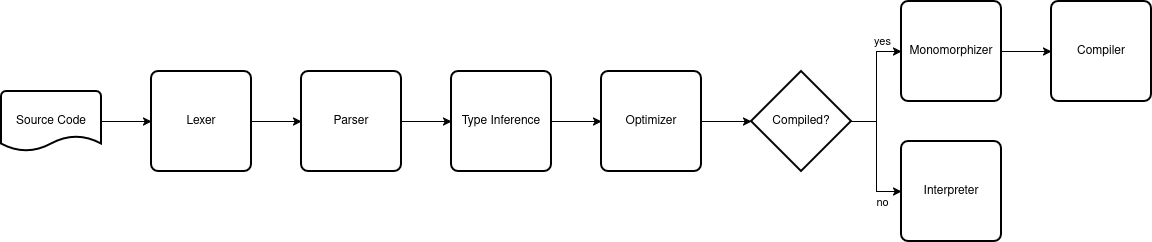
\includegraphics[width=\textwidth]{diagrams/DataFlow.png}
	\caption{Data Flow of the Implementation}
\end{figure}
The data from the file with the source code goes through the lexer,
parser, type inference and optimizer no matter what, and then depending
on if the compiler is chosen it goes through the monomorphizer, whose function will be explained later, and
the compiler instead of the interpreter.
Starting from type inference, this data is transferred fully using the syntax tree,
whereas the lexer gets the source code. Whether the compiler or interpreter is used
is decided by the build script at the time of compilation
of the implementation.

\subsection{The Lexer}
The lexer of the implementations of Imp is a simple single-pass lexer, that computes
the tokens on demand. This is done to avoid memory
allocations other than creating the syntax tree.
Its state consists solely of its
current position in the source text as well as the start
of the current token.

The tokens generated contain full information
about their location in the source code.

\subsubsection{Token Types}
The types of tokens that are returned by the lexer are:
\begin{itemize}
	\item The Keywords \texttt{let} and \texttt{in}, \texttt{lambda}, \texttt{if}, \texttt{then} and \texttt{else},
	      \texttt{case} and \texttt{of}, \texttt{or} and \texttt{and},
	\item the special characters \texttt{.}, \texttt{=}, \texttt{:}, \texttt{(} and \texttt{)}, \texttt{[} and \texttt{]}
	\item the special sequences \texttt{->} and \texttt{=>},
	\item all operators for comparison and mathematical operations,
	      and the special operator \texttt{;} which discards the first argument (useful for side-effects),
	\item Numbers, Booleans, Characters and Strings,
	\item Identifiers, which start with a letter and
	      then continue using alphanumeric characters or underscores,
	\item and Special Tokens for new lines and the end of the file
\end{itemize}

This means that all keywords are reserved and cannot be used
for the name of a variable.

\subsection{The Parser}
\importListing{code/expressions.tex}

The Parser mostly consists of a pretty straight-forward implementation of the Pratt Parsing algorithm
\autocite{prattTopOperatorPrecedence1973}.
This is used for the expressions as shown in Listing \ref{listing:expressions}.
The statements are parsed in a simple loop, as statements cannot be nested in this language.

The two lookup tables that are described in the original paper are represented
in this implementation as functions,
\texttt{getNud} and \texttt{getLed}.
They describe what to do in case the token is found at the start in the case of \texttt{getNud},
or in the middle of an expression in the case of \texttt{getLed}, roughly equivalent to
prefix and infix/postfix operators.

The variable left is filled at each point with the current parsed expression
and is substituted in a loop, if the precedence of the next operator is high enough (line 19).
This check is needed to ensure correct operator precedence.

The problem that there might not be an entry is solved by returning null
in that case. The case of null is handled in both cases by an \texttt{orelse}.
If the result of \texttt{getNud} is null, an error is thrown and returned on lines 5-11 of this excerpt.
However, if \texttt{getLed} returns null, then this does not cause an error, but the currently parsed value of
left is returned.

Precedence for operators is the following:
The highest precedence of all operators is assigned to the \texttt{\^} operator for exponentiation,
followed by \texttt{*} and \texttt{/}, which have equal precedence and finally \texttt{+} and \texttt{-} with equal
precedence as well. This is done to match the precedence conventions of mathematics.
Following these mathematic operators in precedence are the comparison operators
\texttt{<}, \texttt{<=}, \texttt{==}, \texttt{>=}, and \texttt{>}, all with the same precedence.
After these comparisons, the logical operators \texttt{and} and \texttt{or} follow,
so comparisons can be combined with them without brackets.
The lowest precedence of all operators is assigned to \texttt{;}.

\texttt{getLed} however also has the special case that all token types that are present in \texttt{getNud}
can be the start of an argument given to the expression parsed before, since calls are
made just by having two expressions next to each other.
This special rule has the highest precedence of all expression types
so that the result of two functions can be combined using an operator without parentheses.

\subsection{Type Checking/Inference}
The type checker is implemented close to the Algorithm J as described
by Damas and Milner\autocite{damasPrincipalTypeschemesFunctional1982}.
There is however a significant difference to the original type system:
There exists a special type Number(a), which represents either a Float or an Int
and therefore can be unified with both. When unified, the runtime representation
is then Number(Int) or Number(Float).

\importListing{code/unify.tex}

This logic is contained in the unification function outlined
in listing \ref{listing:unify} on line 18-19. It takes advantage of the logic
on lines 3-12 which unify a generic type variable with any type.

The constraint Number(a) is printed similarly to how Type Class
constraints are shown in Haskell, namely the type Number(a) is printed as
\texttt{Number a => a}.

The most significant change to the Algorithm J itself however
lies in the fact that in order to be able
to compute free type variables, meaning independent variables for generalization
faster, levels as described in \autocite{EfficientInsightfulGeneralization2022} are
used. Generalization is the process of finding the free, independent type variables $\vec{a}$ such that the
type of a variable can be described as $\forall\vec{a}.\tau$, thus enabling polymorphism.
The levels are called depth in the code.
These levels are assigned to new type variables based on how many let statements and expressions
deep the algorithm is currently and are adjusted if unified with a variable of lesser depth.
Intuitively, if a type variable contained in the type of a variable assigned via a let statement or expression
has a higher depth than at the start of parsing that statement or expression, the type must have been created
in the declaration itself and cannot have existed outside the current scope, otherwise
the depth would be less. This is equivalent to the notion of
a free type variable.

\subsection{Desugaring}
The \gls{sugar} for linked lists being written as \texttt{[x, y, z, ...]} is now
removed by replacing it with calls to \texttt{Cons} and \texttt{Nil}. This means that e.g.
\texttt{[1, 2]} becomes \texttt{Cons\;1\;(Cons\;2\;Nil)}. This is so that both the interpreter and
the compiler do not need additional functionality for this. The same is done
for strings as \texttt{"xyz..."}, as in the syntax tree both are represented
the same way.

\subsection{The Optimizer}
\importListing{code/optimizer.tex}
The optimizer applies different optimizations depending on whether
the code is interpreted or compiled. When interpreted
the optimizer combines lambdas into a sort of multi-argument function
and combines calls into multi-argument calls.
This is done such that if the multi-argument functions are called with several arguments
at once there is no need for intermediate objects allocated.
The compiler cannot work with this representation as the above optimization needs runtime information
about the number of arguments of a function, which the compiler would need static analysis for.
However, in both cases a list of bound variables is gathered per lambda expression
to optimize the memory consumption of closures as they do not need to clone all values.
Both optimizations' run functions consists of a switch statement handling
the 15 possible types of expressions and running the optimization on the expressions contained
within.

\subsection{The Interpreter}
The interpreter is a simple tree-walking interpreter.
It keeps track of the function calls where the execution is currently located
(the call stack) using both the builtin call stack by Zig through recursion
and a linked list containing the functions name and a hash map (also known as dictionary) mapping the variables to their
respective values in each functions scope.

The most important optimization it employs is proper tail call elimination,
meaning it does not make another stack frame if a function call is the last
thing a function does, making recursion feasible through
tail recursion. This function does not need to be the function whose body the
execution is currently in. This is done by having the evaluation of an expression return
the next part of the syntax tree to evaluate, which is then repeatedly evaluated in a loop until the final result
is reached, avoiding additional elements on the call stack. This method is similar to
a 'trampoline' as used in some variations of Lisp.

\subsection{The Monomorphizer}
The monomorphizer is only used when compiling.
It aims to remove all polymorphism,
needed because LLVM does not allow polymorphism.
To reach that goal it first replaces all instances of free type variables
with the type of Int. In this case, type variables are also considered
bound or non-free if they are in a $\forall$. This is necessary because for example the empty list
can have the type of $List\:a$ for any $a$, but the conversion to \Gls{llvm} \Gls{ir} later on still needs a concrete
type to determine the correct representation.

Once this replacement is done, it eliminates the polymorphism by duplicating
the value assigned to each \texttt{let} for each type it takes the form of
in the code of the program. This can only be done because
in the Hindley-Milner type system, every value
can only be used as a finite number of types.

The whole transformation is done by a simple pass over the syntax tree, gathering
all the types a value takes the form of in the body of each let expression,
or in the rest of the file, in case of a let statement or a type declaration,
getting the instantiation of the $\forall\vec{a}$ back by comparing the generic
with the specific type. For example if the generic type was $\forall a. a \rightarrow a$ and
the type in the body is $Int \rightarrow Int$, the instantiation of the variable $a$ is $Int$.
While doing this, the usages of the variable are changed to refer to a new variable name,
unique to each instantiation.
Once all instantiations are gathered, it copies the syntax tree of the definition once each.

This is essentially the method the programming language implementation MLTon uses.\autocite{Monomorphise}

\subsection{The Compiler}
The Compiler then converts this
monomorphic syntax tree into \Gls{llvm} \Gls{ir} using the C \Gls{api} of LLVM, which
makes the creation of LLVM IR possible from C instead of C++ through
Zigs automatically generated \Gls{ffi}. Zigs \Gls{ffi} allows it to call
C functions directly by automatically generating the correct bindings using the
headers.

Closures are represented in the \Gls{ir} as a struct consisting of two pointers:
The first being the function pointer, the second being a pointer to the heap
where all bound variables are stored.

The functions generated and pointed to in the closure
take two arguments each: Their actual argument
as declared by the source code, and the environment that had been stored
at the time of the closures creation.

Here, little is done to optimize the \Gls{ir} created apart
from recursive calls being done directly instead of through an indirect
call as all other function calls are done, in order to enable
the tail recursion optimization of LLVM itself as it could not recognize the indirect function call
as a recursive call since it would be given via an argument and therefore
could theoretically be different.

Then clang is called on the \Gls{ir}, linking it with a very small library of built-in
functions with the highest optimization level of -O3. As a result, the compiler requires
clang to be present and on the search path of the shell.

\section{Results}
\subsection{Fibonacci Program}
Too see how programs in this language look like, the following program that generates the fibonacci sequence,
will be explained.

\importListing{code/fibonacci.tex}

In this example, the fibonacci sequence is computed in the function
\texttt{fibonacciHelper} through tail recursion. Because of that, that function
can be viewed as a loop which changes the variables \texttt{previous}, \texttt{current} and
\texttt{n} on each iteration. This change is done on line 6.

Throughout its execution, it also prints the current fibonacci number
computed using the two built-in functions \texttt{showInt} and \texttt{print}.

Several expressions are separated by a semicolon (\texttt{;}) which is an operator
in this language that simply discards the result on the left, meaning
the expression on the left is only there for its side-effects like printing.

The main function takes a dummy argument x, because in Imp, there are no
functions that take no argument. This function is then called
after all definitions have been executed.
On line 17 it then reads the number of elements requested,
which is then parsed. As this can fail, this returns a
value of type Option. The case expression then evaluates either line
18, if the parse failed, which just repeats the main function,
or it puts the result into the variable n which is then used in
lines 20-23. Finally on line 24, Void is returned, since Imp functions
also need to return exactly one value.

This example also demonstrates the power of Hindley-Milner type inference,
because no types ever needed to be annotated for the code to work,
but it is still guaranteed that the whole program has no type errors.
The type given to \texttt{fibonacciHelper} is only there for clarity.

Other examples of Imp code can be found in the folder \file{examples} in
the source code.

\subsection{LLVM Transformation}

Additionally, to get a view of how the LLVM IR transformation works, here is
an example of the resulting IR of a simple function,
though cleaned up to remove clutter and add meaningful names.

\begin{minipage}{\linewidth}
	\begin{lstlisting}[
	% there are many more options of styling, see the official documentation, these are just the defaults I like
	frame=single, % make single-line frame around the verbatim
	framesep=2mm, % put some more spacing between the frame and text
	aboveskip=5mm, % put some more space above the box
	basicstyle={\linespread{0.9}\small\ttfamily}, % use typewriter (monospace) font
	caption={Add function in Imp}, % set the caption text
	captionpos=b, % put the caption at the bottom (b) or top (t) or both (bt)
    label={listing:addImp}, % label to be referenced via \ref{}
	numbers=left, % line numbers on the left
	numberstyle={\scriptsize\ttfamily\color{black!60}}, % the style for line numbers
	escapeinside={<@}{@>} % between those sequences are commands evaluated
]
<@\textcolor[HTML]{3010CF}{\textit{\textbf{\texttt{let}}}}@><@\textcolor[HTML]{000000}{\texttt{\ }}@><@\textcolor[HTML]{255CFF}{\texttt{add}}@><@\textcolor[HTML]{000000}{\texttt{:\ }}@><@\textcolor[HTML]{1F8F42}{\texttt{Int\ ->\ Int\ ->\ Int}}@><@\textcolor[HTML]{000000}{\texttt{\ }}@><@\textcolor[HTML]{1041FF}{\texttt{=}}@>
<@\textcolor[HTML]{000000}{\texttt{\ \ \ \ }}@><@\textcolor[HTML]{3010CF}{\textit{\textbf{\texttt{lambda}}}}@><@\textcolor[HTML]{000000}{\texttt{\ }}@><@\textcolor[HTML]{EA5110}{\textit{\texttt{x}}}@><@\textcolor[HTML]{1041FF}{\texttt{.}}@><@\textcolor[HTML]{000000}{\texttt{\ }}@><@\textcolor[HTML]{3010CF}{\textit{\textbf{\texttt{lambda}}}}@><@\textcolor[HTML]{000000}{\texttt{\ }}@><@\textcolor[HTML]{EA5110}{\textit{\texttt{y}}}@><@\textcolor[HTML]{1041FF}{\texttt{.}}@>
<@\textcolor[HTML]{000000}{\texttt{\ \ \ \ \ \ \ \ }}@><@\textcolor[HTML]{EA5110}{\textit{\texttt{x}}}@><@\textcolor[HTML]{000000}{\texttt{\ }}@><@\textcolor[HTML]{1041FF}{\texttt{+}}@><@\textcolor[HTML]{000000}{\texttt{\ }}@><@\textcolor[HTML]{EA5110}{\textit{\texttt{y}}}@>

\end{lstlisting}
	\begin{lstlisting}[
	% there are many more options of styling, see the official documentation, these are just the defaults I like
	frame=single, % make single-line frame around the verbatim
	framesep=2mm, % put some more spacing between the frame and text
	aboveskip=5mm, % put some more space above the box
	basicstyle={\linespread{0.9}\small\ttfamily}, % use typewriter (monospace) font
	caption={Add function compiled to LLVM IR}, % set the caption text
	captionpos=b, % put the caption at the bottom (b) or top (t) or both (bt)
    label={listing:addLLVM}, % label to be referenced via \ref{}
	numbers=left, % line numbers on the left
	numberstyle={\scriptsize\ttfamily\color{black!60}}, % the style for line numbers
	escapeinside={<@}{@>} % between those sequences are commands evaluated
]
<@\textcolor[HTML]{3010CF}{\textbf{\texttt{define}}}@><@\textcolor[HTML]{000000}{\texttt{\ }}@><@\textcolor[HTML]{FF1010}{\texttt{\{}}@><@\textcolor[HTML]{1F8F42}{\texttt{\ }}@><@\textcolor[HTML]{10909F}{\texttt{ptr}}@><@\textcolor[HTML]{1041FF}{\texttt{,}}@><@\textcolor[HTML]{1F8F42}{\texttt{\ }}@><@\textcolor[HTML]{10909F}{\texttt{ptr}}@><@\textcolor[HTML]{1F8F42}{\texttt{\ }}@><@\textcolor[HTML]{FF1010}{\texttt{\}}}@><@\textcolor[HTML]{000000}{\texttt{\ }}@><@\textcolor[HTML]{000000}{\texttt{@add}}@><@\textcolor[HTML]{FF1010}{\texttt{(}}@><@\textcolor[HTML]{10909F}{\texttt{i64}}@><@\textcolor[HTML]{EA5110}{\textit{\texttt{\ }}}@><@\textcolor[HTML]{000000}{\texttt{\%x}}@><@\textcolor[HTML]{1041FF}{\texttt{,}}@><@\textcolor[HTML]{000000}{\texttt{\ }}@><@\textcolor[HTML]{10909F}{\texttt{ptr}}@><@\textcolor[HTML]{EA5110}{\textit{\texttt{\ }}}@><@\textcolor[HTML]{000000}{\texttt{\%bound}}@><@\textcolor[HTML]{FF1010}{\texttt{)}}@><@\textcolor[HTML]{000000}{\texttt{\ }}@><@\textcolor[HTML]{FF1010}{\texttt{\{}}@>
<@\textcolor[HTML]{7777BB}{\texttt{entry:}}@>
<@\textcolor[HTML]{000000}{\texttt{\ \ }}@><@\textcolor[HTML]{000000}{\texttt{\%int\_ptr}}@><@\textcolor[HTML]{000000}{\texttt{\ }}@><@\textcolor[HTML]{1041FF}{\texttt{=}}@><@\textcolor[HTML]{000000}{\texttt{\ }}@><@\textcolor[HTML]{1010FF}{\texttt{getelementptr}}@><@\textcolor[HTML]{000000}{\texttt{\ }}@><@\textcolor[HTML]{FF1010}{\texttt{\{}}@><@\textcolor[HTML]{1F8F42}{\texttt{\ }}@><@\textcolor[HTML]{10909F}{\texttt{i64}}@><@\textcolor[HTML]{1F8F42}{\texttt{\ }}@><@\textcolor[HTML]{FF1010}{\texttt{\}}}@><@\textcolor[HTML]{1041FF}{\texttt{,}}@><@\textcolor[HTML]{000000}{\texttt{\ }}@><@\textcolor[HTML]{10909F}{\texttt{ptr}}@><@\textcolor[HTML]{000000}{\texttt{\ }}@><@\textcolor[HTML]{EA5110}{\textit{\texttt{null}}}@><@\textcolor[HTML]{1041FF}{\texttt{,}}@><@\textcolor[HTML]{000000}{\texttt{\ }}@><@\textcolor[HTML]{10909F}{\texttt{i32}}@><@\textcolor[HTML]{000000}{\texttt{\ }}@><@\textcolor[HTML]{EA5110}{\texttt{1}}@>
<@\textcolor[HTML]{000000}{\texttt{\ \ }}@><@\textcolor[HTML]{000000}{\texttt{\%sizeof\_int}}@><@\textcolor[HTML]{000000}{\texttt{\ }}@><@\textcolor[HTML]{1041FF}{\texttt{=}}@><@\textcolor[HTML]{000000}{\texttt{\ }}@><@\textcolor[HTML]{1010FF}{\texttt{ptrtoint}}@><@\textcolor[HTML]{000000}{\texttt{\ }}@><@\textcolor[HTML]{10909F}{\texttt{ptr}}@><@\textcolor[HTML]{000000}{\texttt{\ }}@><@\textcolor[HTML]{000000}{\texttt{\%int\_ptr}}@><@\textcolor[HTML]{000000}{\texttt{\ }}@><@\textcolor[HTML]{3010CF}{\textit{\textbf{\texttt{to}}}}@><@\textcolor[HTML]{000000}{\texttt{\ }}@><@\textcolor[HTML]{10909F}{\texttt{i64}}@>
<@\textcolor[HTML]{000000}{\texttt{\ \ }}@><@\textcolor[HTML]{000000}{\texttt{\%new\_bound}}@><@\textcolor[HTML]{000000}{\texttt{\ }}@><@\textcolor[HTML]{1041FF}{\texttt{=}}@><@\textcolor[HTML]{000000}{\texttt{\ }}@><@\textcolor[HTML]{1010FF}{\texttt{call}}@><@\textcolor[HTML]{000000}{\texttt{\ }}@><@\textcolor[HTML]{10909F}{\texttt{ptr}}@><@\textcolor[HTML]{000000}{\texttt{\ }}@><@\textcolor[HTML]{000000}{\texttt{@GC\_malloc}}@><@\textcolor[HTML]{FF1010}{\texttt{(}}@><@\textcolor[HTML]{10909F}{\texttt{i64}}@><@\textcolor[HTML]{EA5110}{\textit{\texttt{\ }}}@><@\textcolor[HTML]{000000}{\texttt{\%sizeof\_int}}@><@\textcolor[HTML]{FF1010}{\texttt{)}}@>
<@\textcolor[HTML]{000000}{\texttt{\ \ }}@><@\textcolor[HTML]{000000}{\texttt{\%x\_location}}@><@\textcolor[HTML]{000000}{\texttt{\ }}@><@\textcolor[HTML]{1041FF}{\texttt{=}}@><@\textcolor[HTML]{000000}{\texttt{\ }}@><@\textcolor[HTML]{1010FF}{\texttt{getelementptr}}@><@\textcolor[HTML]{000000}{\texttt{\ }}@><@\textcolor[HTML]{FF1010}{\texttt{\{}}@><@\textcolor[HTML]{1F8F42}{\texttt{\ }}@><@\textcolor[HTML]{10909F}{\texttt{i64}}@><@\textcolor[HTML]{1F8F42}{\texttt{\ }}@><@\textcolor[HTML]{FF1010}{\texttt{\}}}@><@\textcolor[HTML]{1041FF}{\texttt{,}}@><@\textcolor[HTML]{000000}{\texttt{\ }}@><@\textcolor[HTML]{10909F}{\texttt{ptr}}@><@\textcolor[HTML]{000000}{\texttt{\ }}@><@\textcolor[HTML]{000000}{\texttt{\%new\_bound}}@><@\textcolor[HTML]{1041FF}{\texttt{,}}@><@\textcolor[HTML]{000000}{\texttt{\ }}@><@\textcolor[HTML]{10909F}{\texttt{i32}}@><@\textcolor[HTML]{000000}{\texttt{\ }}@><@\textcolor[HTML]{EA5110}{\texttt{0}}@><@\textcolor[HTML]{1041FF}{\texttt{,}}@><@\textcolor[HTML]{000000}{\texttt{\ }}@><@\textcolor[HTML]{10909F}{\texttt{i32}}@><@\textcolor[HTML]{000000}{\texttt{\ }}@><@\textcolor[HTML]{EA5110}{\texttt{0}}@>
<@\textcolor[HTML]{000000}{\texttt{\ \ }}@><@\textcolor[HTML]{1010FF}{\texttt{store}}@><@\textcolor[HTML]{000000}{\texttt{\ }}@><@\textcolor[HTML]{10909F}{\texttt{i64}}@><@\textcolor[HTML]{000000}{\texttt{\ }}@><@\textcolor[HTML]{000000}{\texttt{\%x}}@><@\textcolor[HTML]{1041FF}{\texttt{,}}@><@\textcolor[HTML]{000000}{\texttt{\ }}@><@\textcolor[HTML]{10909F}{\texttt{ptr}}@><@\textcolor[HTML]{000000}{\texttt{\ }}@><@\textcolor[HTML]{000000}{\texttt{\%x\_location}}@>
<@\textcolor[HTML]{000000}{\texttt{\ \ }}@><@\textcolor[HTML]{000000}{\texttt{\%add\_const\_closure}}@><@\textcolor[HTML]{000000}{\texttt{\ }}@><@\textcolor[HTML]{1041FF}{\texttt{=}}@><@\textcolor[HTML]{000000}{\texttt{\ }}@><@\textcolor[HTML]{1010FF}{\texttt{insertvalue}}@><@\textcolor[HTML]{000000}{\texttt{\ }}@><@\textcolor[HTML]{FF1010}{\texttt{\{}}@><@\textcolor[HTML]{1F8F42}{\texttt{\ }}@><@\textcolor[HTML]{10909F}{\texttt{ptr}}@><@\textcolor[HTML]{1041FF}{\texttt{,}}@><@\textcolor[HTML]{1F8F42}{\texttt{\ }}@><@\textcolor[HTML]{10909F}{\texttt{ptr}}@><@\textcolor[HTML]{1F8F42}{\texttt{\ }}@><@\textcolor[HTML]{FF1010}{\texttt{\}}}@><@\textcolor[HTML]{000000}{\texttt{\ }}@><@\textcolor[HTML]{FF1010}{\texttt{\{}}@><@\textcolor[HTML]{724BFF}{\textit{\texttt{\ }}}@><@\textcolor[HTML]{10909F}{\texttt{ptr}}@><@\textcolor[HTML]{724BFF}{\textit{\texttt{\ }}}@><@\textcolor[HTML]{000000}{\texttt{@add\_const}}@><@\textcolor[HTML]{1041FF}{\texttt{,}}@><@\textcolor[HTML]{724BFF}{\textit{\texttt{\ }}}@><@\textcolor[HTML]{10909F}{\texttt{ptr}}@><@\textcolor[HTML]{724BFF}{\textit{\texttt{\ }}}@><@\textcolor[HTML]{EA5110}{\textit{\texttt{undef}}}@><@\textcolor[HTML]{724BFF}{\textit{\texttt{\ }}}@><@\textcolor[HTML]{FF1010}{\texttt{\}}}@><@\textcolor[HTML]{1041FF}{\texttt{,}}@><@\textcolor[HTML]{000000}{\texttt{\ }}@><@\textcolor[HTML]{10909F}{\texttt{ptr}}@><@\textcolor[HTML]{000000}{\texttt{\ }}@><@\textcolor[HTML]{000000}{\texttt{\%new\_bound}}@><@\textcolor[HTML]{1041FF}{\texttt{,}}@><@\textcolor[HTML]{000000}{\texttt{\ }}@><@\textcolor[HTML]{EA5110}{\texttt{1}}@>
<@\textcolor[HTML]{000000}{\texttt{\ \ }}@><@\textcolor[HTML]{1010FF}{\textit{\texttt{ret}}}@><@\textcolor[HTML]{000000}{\texttt{\ }}@><@\textcolor[HTML]{FF1010}{\texttt{\{}}@><@\textcolor[HTML]{1F8F42}{\texttt{\ }}@><@\textcolor[HTML]{10909F}{\texttt{ptr}}@><@\textcolor[HTML]{1041FF}{\texttt{,}}@><@\textcolor[HTML]{1F8F42}{\texttt{\ }}@><@\textcolor[HTML]{10909F}{\texttt{ptr}}@><@\textcolor[HTML]{1F8F42}{\texttt{\ }}@><@\textcolor[HTML]{FF1010}{\texttt{\}}}@><@\textcolor[HTML]{000000}{\texttt{\ }}@><@\textcolor[HTML]{000000}{\texttt{\%add\_const\_closure}}@>
<@\textcolor[HTML]{FF1010}{\texttt{\}}}@>

<@\textcolor[HTML]{3010CF}{\textbf{\texttt{define}}}@><@\textcolor[HTML]{000000}{\texttt{\ }}@><@\textcolor[HTML]{10909F}{\texttt{i64}}@><@\textcolor[HTML]{000000}{\texttt{\ }}@><@\textcolor[HTML]{000000}{\texttt{@add\_const}}@><@\textcolor[HTML]{FF1010}{\texttt{(}}@><@\textcolor[HTML]{10909F}{\texttt{i64}}@><@\textcolor[HTML]{EA5110}{\textit{\texttt{\ }}}@><@\textcolor[HTML]{000000}{\texttt{\%y}}@><@\textcolor[HTML]{1041FF}{\texttt{,}}@><@\textcolor[HTML]{000000}{\texttt{\ }}@><@\textcolor[HTML]{10909F}{\texttt{ptr}}@><@\textcolor[HTML]{EA5110}{\textit{\texttt{\ }}}@><@\textcolor[HTML]{000000}{\texttt{\%bound}}@><@\textcolor[HTML]{FF1010}{\texttt{)}}@><@\textcolor[HTML]{000000}{\texttt{\ }}@><@\textcolor[HTML]{FF1010}{\texttt{\{}}@>
<@\textcolor[HTML]{7777BB}{\texttt{entry:}}@>
<@\textcolor[HTML]{000000}{\texttt{\ \ }}@><@\textcolor[HTML]{000000}{\texttt{\%x\_location}}@><@\textcolor[HTML]{000000}{\texttt{\ }}@><@\textcolor[HTML]{1041FF}{\texttt{=}}@><@\textcolor[HTML]{000000}{\texttt{\ }}@><@\textcolor[HTML]{1010FF}{\texttt{getelementptr}}@><@\textcolor[HTML]{000000}{\texttt{\ }}@><@\textcolor[HTML]{FF1010}{\texttt{\{}}@><@\textcolor[HTML]{1F8F42}{\texttt{\ }}@><@\textcolor[HTML]{10909F}{\texttt{i64}}@><@\textcolor[HTML]{1F8F42}{\texttt{\ }}@><@\textcolor[HTML]{FF1010}{\texttt{\}}}@><@\textcolor[HTML]{1041FF}{\texttt{,}}@><@\textcolor[HTML]{000000}{\texttt{\ }}@><@\textcolor[HTML]{10909F}{\texttt{ptr}}@><@\textcolor[HTML]{000000}{\texttt{\ }}@><@\textcolor[HTML]{000000}{\texttt{\%bound}}@><@\textcolor[HTML]{1041FF}{\texttt{,}}@><@\textcolor[HTML]{000000}{\texttt{\ }}@><@\textcolor[HTML]{10909F}{\texttt{i32}}@><@\textcolor[HTML]{000000}{\texttt{\ }}@><@\textcolor[HTML]{EA5110}{\texttt{0}}@><@\textcolor[HTML]{1041FF}{\texttt{,}}@><@\textcolor[HTML]{000000}{\texttt{\ }}@><@\textcolor[HTML]{10909F}{\texttt{i32}}@><@\textcolor[HTML]{000000}{\texttt{\ }}@><@\textcolor[HTML]{EA5110}{\texttt{0}}@>
<@\textcolor[HTML]{000000}{\texttt{\ \ }}@><@\textcolor[HTML]{000000}{\texttt{\%x}}@><@\textcolor[HTML]{000000}{\texttt{\ }}@><@\textcolor[HTML]{1041FF}{\texttt{=}}@><@\textcolor[HTML]{000000}{\texttt{\ }}@><@\textcolor[HTML]{1010FF}{\texttt{load}}@><@\textcolor[HTML]{000000}{\texttt{\ }}@><@\textcolor[HTML]{10909F}{\texttt{i64}}@><@\textcolor[HTML]{1041FF}{\texttt{,}}@><@\textcolor[HTML]{000000}{\texttt{\ }}@><@\textcolor[HTML]{10909F}{\texttt{ptr}}@><@\textcolor[HTML]{000000}{\texttt{\ }}@><@\textcolor[HTML]{000000}{\texttt{\%x\_location}}@>
<@\textcolor[HTML]{000000}{\texttt{\ \ }}@><@\textcolor[HTML]{000000}{\texttt{\%result}}@><@\textcolor[HTML]{000000}{\texttt{\ }}@><@\textcolor[HTML]{1041FF}{\texttt{=}}@><@\textcolor[HTML]{000000}{\texttt{\ }}@><@\textcolor[HTML]{1010FF}{\texttt{add}}@><@\textcolor[HTML]{000000}{\texttt{\ }}@><@\textcolor[HTML]{10909F}{\texttt{i64}}@><@\textcolor[HTML]{000000}{\texttt{\ }}@><@\textcolor[HTML]{000000}{\texttt{\%x}}@><@\textcolor[HTML]{1041FF}{\texttt{,}}@><@\textcolor[HTML]{000000}{\texttt{\ }}@><@\textcolor[HTML]{000000}{\texttt{\%y}}@>
<@\textcolor[HTML]{000000}{\texttt{\ \ }}@><@\textcolor[HTML]{1010FF}{\textit{\texttt{ret}}}@><@\textcolor[HTML]{000000}{\texttt{\ }}@><@\textcolor[HTML]{10909F}{\texttt{i64}}@><@\textcolor[HTML]{000000}{\texttt{\ }}@><@\textcolor[HTML]{000000}{\texttt{\%result}}@>
<@\textcolor[HTML]{FF1010}{\texttt{\}}}@>

\end{lstlisting}

\end{minipage}

The first lambda defined on line 2 of Listing \ref{listing:addImp} got transformed
into the function \texttt{@add} of Listing \ref{listing:addLLVM}.
As the second lambda binds the value of \texttt{x}, \texttt{@add} allocates
enough memory to store it on lines 3-5, then gets the exact location on line 6, which
is done since there might be more than one bound variable, but in this case is redundant.
Line 7 then stores \texttt{x} while line 8 creates the closure by inserting the pointer to the bound
variable in a struct.
Finally on line 9, the closure is returned.

The function \texttt{@add\_const} then accesses this bound variable, again first getting the
location on the redundant line 14, then loads the actual value of \texttt{x} on line 15
and finally computes the result on line 16 which is returned on line 17.

\subsection{Benchmark}

To compare the performance of the two implementations with a real-world language,
a small benchmark was run using a tool called hyperfine\autocite{peterHyperfine2023}.
It gathers its data by running a specific command several times and calculates
the statistical measures.
Both the Imp and the Python implementation compute and print the mandelbrot set.
For the compiler, only the compiled program was benchmarked, and not
the time it takes to compile it. The version of LLVM used was 20.1.8.
The Python implementation was run using CPython 3.12.1.
All the files being benchmarked can be found in the folder \path{benchmark}.

\begin{table}[H]
	\centering
	\begin{tabular}{|l|l|l|l|}
		\hline
		Language             & Mean and $\sigma$ [ms] & Min [ms] & Max [ms] \\ \hline
		Imp with Compiler    & 9.7 ± 2.7              & 5.3      & 16.9     \\ \hline
		Imp with Interpreter & 390.1 ± 16.9           & 362.2    & 421.2    \\ \hline
		Python               & 57.9 ± 8.0             & 40.1     & 73.7     \\ \hline
	\end{tabular}
\end{table}

As can be seen in this table, the language Imp is slower than Python in this case if interpreted,
but the compiler brought an improvement of approximately 40x over the interpreter, while Python
takes almost 6 times the time that the compiled program takes.

\section{Discussion}
As seen in the example given, the language
can be used for mathematical computation.
Both the interpreter and compiler are also relatively fast and
(with a minor caveat) memory-safe. The feasability of this method of
compilation was shown by the benchmark.

\subsection{Shortcomings}\label{shortcomings}
The language Imp is a functioning prototype, but there are several
aspects which would need to be treated in order for this language
to be useful for any practical purposes.

\subsubsection{Input/output}
Input/output is an essential part of any programming language.
The language Imp is no exception to this, having the two functions
\texttt{print} and \texttt{read} which print to standard output and read from
standard input respectively. However, there is currently no way
to read from or write to files, which is essential for a program
to store information for later usages of it or to load and/or output larger
amounts of information.

To enable this feature, a type for Files or Buffers would have to be
introduced for fast, type-safe interaction.

\subsubsection{Library System}
In Imp, it is impossible to import other files from a program.
This would be essential for the development of libraries.
To enable imports and therefore libraries, a topological sorting
algorithm could be used, since the order of definitions does
matter in this language and circular references cannot exist.

This would enable a much more practical implementation of the standard
library as well, since e.g. functions that operate on functions could be used
in almost all other parts of the library.

\subsubsection{FFI}
At the moment, Imp cannot access system libraries or libraries
written in other languages at all, meaning GUIs or even most TUIs
(terminal user interfaces) are impossible to create,
since you could not use libraries like QT.

This could be mitigated by a large set of built-in functions based
on which a standard library could be built, or more simply, though
less securely, using an FFI (foreign function interface).

Using a foreign function interface, one could declare functions that
exist in another language (most likely C), and their types and then use
those functions. This would lead to other challenges however, since
there exists no equivalent to many of the types in C.
The types would however need to match up exactly,
putting a huge burden on the programmer writing the declarations
as there should be no type errors, otherwise the whole type system
would be for nothing, as well as the compiler, as it would no longer
be free to represent its objects however it wants.
LLVM does also not guarantee correct FFI, even if the types
seem to match up.

\subsubsection{OS Compatibility}
As the compiler of this language depends on both
LLVM and Boehm \Gls{gc}, it can only be used on operating systems
that support both. Luckily, Linux, MacOS and Windows all meet these requirements.

Windows however does not have
an officially supported prebuilt package for LLVM which includes the headers as well
as the libraries to be linked and which does not depend on MSVC and its
implementation of the C/C++ standard libraries.

Zig does not compile parts of the code it can easily prove to never be run,
which means that if LLVM is not available it does not prevent compilation and execution of the interpreter
even if the compiler is imported.
Thus it is not needed to create two copies of the project for the interpreter and compiler.
This was not originally intended, but the usage of Zig turned out to be a lucky accident for that matter.

\subsection{Room for improvement}
There are many parts of both the compiler and the
interpreter, which could be improved significantly
for enhanced speed and better memory consumption.

\subsubsection{Garbage Collector}
Though both the compiler and the interpreter produce
garbage collected programs, the compiler uses the
conservative Boehm-Demers-Weiser \Gls{gc} \autocite{GarbageCollector},
which is unaware of any of the types of Imp and therefore
has to assume that anything that could be a pointer,
is in fact a pointer. It should therefore be replaced with
precise \Gls{gc} to prevent leaks caused by values randomly looking
like pointers.
Meanwhile, the interpreter uses a very basic mark-and-sweep
\Gls{gc}. However this could very easily be improved
by using methods like Generational Garbage Collection, where
young objects are checked more often than older ones, which are more
likely to live for the entirety of the program.

\subsubsection{Defunctionalization}
Furthermore, another possible optimization done by almost all
functional programming languages nowadays is some form of
defunctionalization, which is a process which tries
to eliminate functions as arguments, replacing them with
an object that is given as an argument which denotes which
function it represents.

One new interesting approach that seems to be promising
is the technique of lambda set specialization
\autocite{brandonBetterDefunctionalizationLambda2023a}, which
could be applied to this language relatively easily,
since it assumes a Hindley-Milner style type inference
as well.

\section{Conclusions}
In conclusion, the goals were met.
The language is now fully functional and able to be tested by anyone.
There are a few aspects that would need to be improved for it to be
useful for most practical use cases as explained in section \ref{shortcomings},
but it is already a useable language.

The language created can now be used as a starting point for a more
feature-rich language.

\newpage
\printbibliography
\newpage
\lstlistoflistings
\listoffigures

\newpage
\printglossaries

\appendix

\section{Acknowledgement}
Thanks go to my parents, Simon and Marion Giger who have proofread this paper
and my supervisor, Adrian Lüthi who supported me with encouragement and information.

\section{Source Code}
The source code for the compiler and interpreter can be found on
\href{https://github.com/enmiligi/matura-project}{GitHub}.
The tree-sitter parser can be found \href{https://github.com/enmiligi/tree-sitter-imp}{here}
and the extension for Zed enabling syntax highlighting is located \href{https://github.com/enmiligi/zed-imp}{here}.

\end{document}
